\section{Processing Models}
This section describes the various processing data processing models that are possible with
Spring XD, and provides configuration and deployment examples.
Note that this is not an exhaustive list of all
deployment types, see section~\ref{sec:Use Cases} for descriptions of real
world deployments.

\subsection {Streams}

A stream defines the near-real time movement of data from a source (see~\ref{sec:Source}) to a
sink (see~\ref{sec:Sink}), passing through any number of processors (see~\ref{sec:Source}).  Spring XD streams can
also integrate with other event based solutions such as Apache Spark Streaming.

For example, the following stream definition can be used to ingest
MQTT\cite{mqtt} data sent by a number of sensors directly into HDFS:

\begin{lstlisting}
stream create ingest
  --definition "mqtt | hdfs"
\end{lstlisting}

In a more elaborate setting, an application can collect data from
different sources, and Spring XD can provide the means to merge them
in a single stream. The streams \texttt{in-mqtt} and \texttt{in-http}
collect data from sensors via MQTT and HTTP, respectively, and
contribute to a single queue \texttt{hdfs-in}. The merged result
is saved into HDFS.

\begin{lstlisting}
stream create in-mqtt --definition
  "mqtt > queue:hdfs-in"

stream create in-http --definition
  "http > queue:hdfs-in"

stream create ingest --definition
  "queue:hdfs-in > hdfs"
\end{lstlisting}

Processor modules in a stream offer the ability to transform, filter,
and enrich data as it moves from one module to another.  In the example below
the stream will accept data from a http source and filter out any message
that does not have the word ``ocean'' and then transform the message
to all caps:

\begin{lstlisting}
stream create oceanStream
 --definition "http | filter
 --expression=payload.contains('ocean') |
 transform
 --expression=payload.toUpperCase() |
 hdfs"
\end{lstlisting}

In cases that a stream should be deactivated but the definition of the stream
should be maintained, the stream can be \emph{undeployed}:

\begin{lstlisting}
stream undeploy oceanStream
\end{lstlisting}

If the stream is no longer needed it can be \emph{destroyed}:

\begin{lstlisting}
stream destroy oceanStream
\end{lstlisting}

\subsection {Batch Jobs}

Spring XD allows users to create batch workflow solutions that span traditional
use-cases such as moving data between flat files and relational databases as
well as Hadoop use-cases where analysis logic is broken up into several steps
that run on a Hadoop cluster. Spring XD can deploy and launch a Spark application
as a batch job. The following is an example of creating a
job definition in XD (this assumes an existing module job named \emph{sensors} that
implements the processing logic):

\begin{lstlisting}
job create sensorProcess --definition "sensors"
\end{lstlisting}

An important feature of Spring XD is the regular
execution of jobs, as well as the ability to replay older datasets, for
instance reconstructing the data views in case of loss or error.
The following mechanisms are available:

\begin{itemize*}
\item \emph{manual} job launch through its shell user interface or
administrative UI
\item \emph{stream-controlled} where the jobs are launched by a stream of
\emph{trigger} messages
\item \emph{scheduled} job launch according to a \texttt{cron} expression
\end{itemize*}

For example, a job can be launched manually as follows:

\begin{lstlisting}
job launch sensorProcess
\end{lstlisting}

Or, more typically, it can be launched on a schedule:

\begin{lstlisting}
stream create --name launchSensorProcess
  --definition  "trigger --cron=`0/5 * * * * *'
  > queue:job:sensorProcess" --deploy
\end{lstlisting}

\subsection {Combining Streams and Jobs}

Spring XD offers the ability for streams and jobs to work together. Streams
can launch jobs, and streams can receive notifications from a job
as it is executing.  In the example below an http source will pass the http
payload to the ``myHttpJob'', thus launching the job:

\begin{lstlisting}
stream create --name jobStream --definition
  "http > queue:job:myHttpJob" --deploy
\end{lstlisting}

In the example below a stream will receive all events from a job and write
the data to the log:

\begin{lstlisting}
job create --name myHttpJob
 --definition "httpJob" --deploy

stream create --name aggregatedEvents
  --definition "tap:job:myHttpJob >log" --deploy

job launch myHttpJob
\end{lstlisting}

\subsection {Tapping a Stream} \label{sssec:deploytap}

A tap ``listens'' to data in an existing stream and passes it into a separate
stream. The creation and existence of a tap does not modify the stream that
is being tapped. Typically the underlying message bus uses a publish/subscribe
message broker, and follows the \emph{wiretap}~\cite{wiretap}
pattern. The tapped stream is processed concurrently with the main stream, so
 consumers with different speeds downstream from the tapping point do not
 interfere with each other. Taps are recommended as way to collect metrics and perform
analytics on a stream of data. An example of this is shown below where a
tap counts the number of MQTT messages received by a source and sent to an
HDFS sink:

\begin{lstlisting}
stream create ingest
 --definition "mqtt|hdfs" --deploy

stream create ingestTap
 --definition "tap:stream:ingest>counter
 --name=ingestCounter" --deploy
\end{lstlisting}

\subsection {Module Counts and Stream Partitioning}
At deployment time a Spring XD stream can be configured to establish the number
of instances of each module in the stream. For example a stream may contain
a processor that is resource intensive, and needs to be
load balanced across multiple containers. The default
settings for a stream deployment will create one module instance for each
module in the stream definition. In the sample stream below the
deployment will create 3 \emph{data-processor} instances distributed
across 3 containers in the cluster:

\begin{lstlisting}
stream create ingest
  --definition
  "mqtt | data-processor | hdfs"

stream deploy --properties
  "module.data-processor.count=3"
\end{lstlisting}

By default Spring XD will send messages to each of the \emph{data-processor}
instances using round robin logic.

Spring XD streams can be partitioned at deployment time to route messages to the
same module instance based on the contents of the message. One example
would be if the processor aggregates data by ``sensorId'' and this step needs to
run using co-located resources.  An example of this is enumerated below:

\begin{lstlisting}
stream create ingest
 --definition
 "mqtt | data-processor | hdfs"

stream deploy --properties
 "module.jms.producer.partitionKeyExpression=
 payload.sensorId,
 module.data-processor.count=3"
\end{lstlisting}

In this example, instead of round robin processing by the \emph{data-processor}
module, the data passing through the stream will be partitioned by ``sensorId''
across the \emph{data-processor} modules.

\subsection {Reactive Processing}


\emph{Reactive programming} is a programming paradigm centered around asynchronous
stream processing. The central concept is that incoming data can be processed in an
ordered, asynchronous and event-driven manner, using functional operators to describe
transformations that apply to an entire stream of incoming data. Operators can
vary from individual item transformations, to grouping and aggregation over given
time windows, and can be composed into complex data processing pipelines that produce
outbound streams of data.

ReactiveX~\cite{reactivex} is one of the most common set of reactive APIs, centered around
the \texttt{Observable} abstraction of an unbounded stream of asynchronous events,
together with a rich set of operators for composing and transforming them.
RxJava~\cite{rxjava} is the Java implementation of the ReactiveX API.

Spring XD provides support for reactive programming through a special type of
processor that describes the transformations on asynchronous streams of data, as
opposed to focusing on the transformations that occur on discrete events. For example,
an RxJava processor for calculating average values over a sliding time window can look as follows:

\begin{lstlisting}
public class MovingAverage
  implements Processor<Tuple,Tuple> {

  @Override
  public Observable<Tuple>
    process(Observable<Tuple> inputStream) {
    return inputStream
      .map(tuple -> tuple.getDouble("measurement"))
      .window(5,1,SECONDS)
      .flatMap(data -> average(data))
      .map(avg -> tuple().of("average", avg)));
    }
}
\end{lstlisting}

The custom module implements the \texttt{Processor} interface and the
\texttt{process} method, whose role is not to execute transformations
on the individual messages of the stream, but to describe a series of
transformations that will be performed on the items emitted by the
\texttt{Observable}: mapping, windowing and the average calculation.

As shown in figure \ref{fig:rxjava}, Spring XD has the responsibility of transforming the
flow of discrete messages arriving on a processor's input channel into an
RxJava \texttt{Observable}, as well as transforming the \texttt{Observable}
returned by the processor module into a flow of discrete messages sent on
the output channel.

\begin{figure}[ht]
\centering
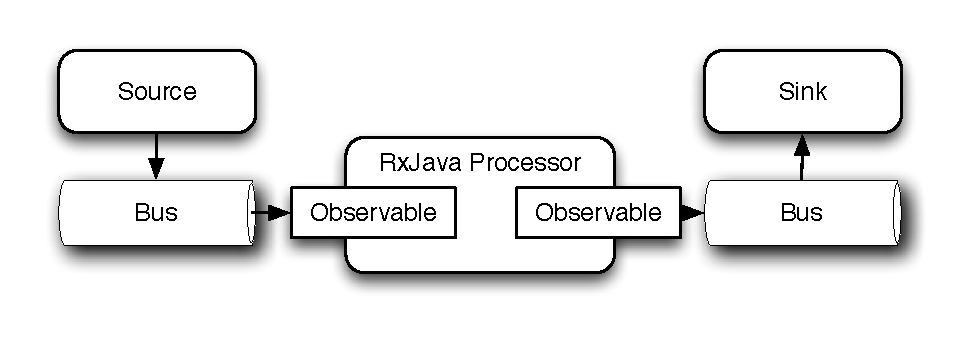
\epsfig{file=rxjava.eps, width=3in}
\caption{Reactive module using RxJava}
\label{fig:rxjava}
\end{figure}

For example, the processor listed above can then be packaged as part of a regular
 processor module (called, for example \emph{averages}) and uses as part of a
 regular stream definition.

\begin{lstlisting}
stream create --name average-sensors
  --definition  "mqtt | averages | log" --deploy
\end{lstlisting}
